\begin{surferPage}[Quintic (15 Cusps)]{منحنى مخمس ذو 15 نتوءاً}
  يملك المنحنى من الدرجة $5$ (مخمس) $15$ متفرداً من النوع $A_2$ (المسماة نتوءات)؛ تم تقديم هذا المنحنى المخمس بالإضافة إلى سلسلة سطوح مرتبطة به في مقالة من 2005 كتبها أوليفر لابس (Oliver Labs).
    خمسة نتوءات تختلف في الشكل عن العشرة الأخرى.
   فهذه النتوءات الخمسة هي متفردات من نوع $A_2^{+-}$ ( للمزيد من المعلومات يمكن مراجعة الجاليريا عن المتفردات البسيطة):

     \vspace*{-0.3em}
    \begin{center}
      \begin{tabular}{c@{\qquad}c}
        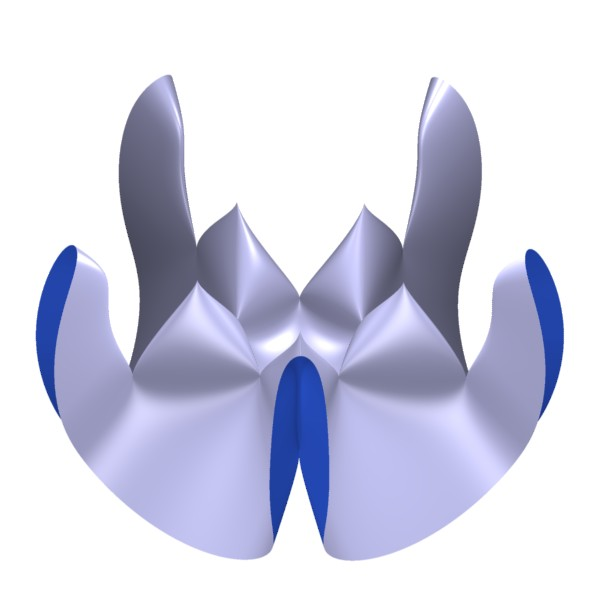
\includegraphics[height=1.2cm]{./../../common/images/dessins_quint_15a2}
        &
        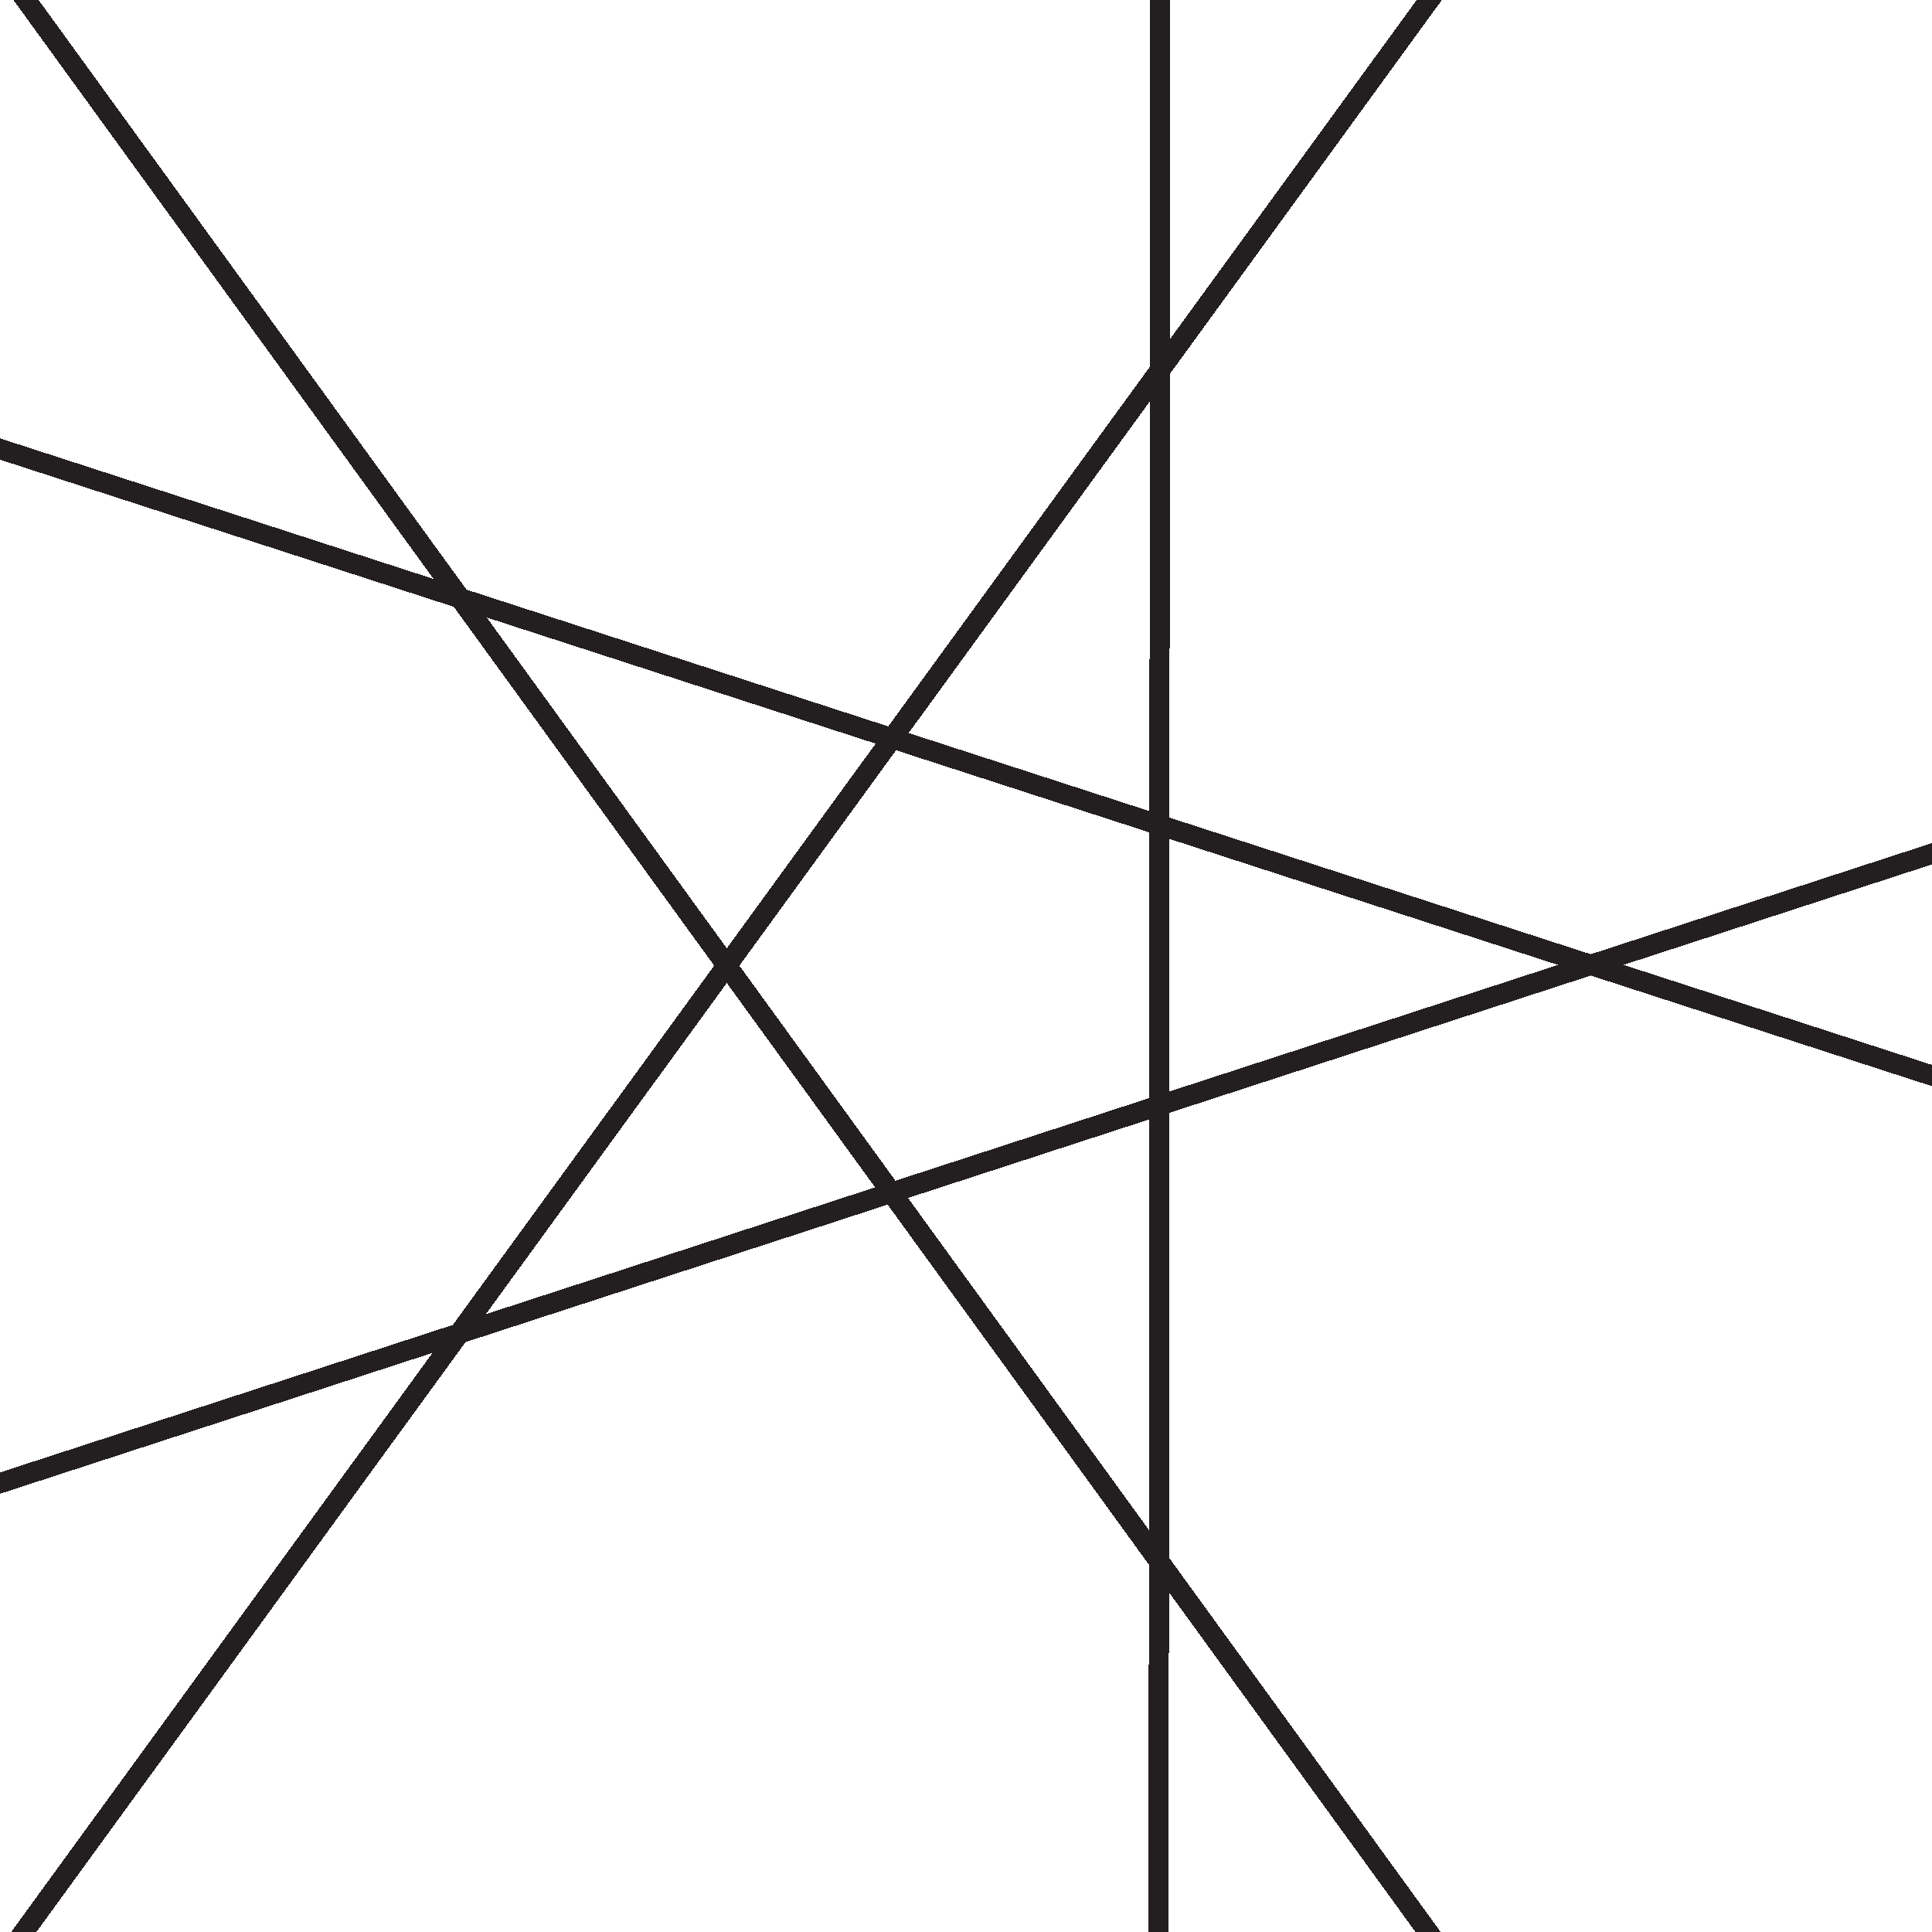
\includegraphics[height=1.2cm]{./../../common/images/rp5.pdf}
      \end{tabular}
    \end{center}
    \vspace*{-0.3em}    
    
    لهذا المنحنى معادلة من الشكل: 
    $S_5(x,y) + t(z)=0,$
    حيث $S_5(x,y)$ هو خماسي أضلاع منتظم (الصورة على اليمين) وحيث  $t(z)$ هو متخالف من متعددات حدود شيبيشيف (Tchebychev polynomials) التي أتينا على ذكرها مرات عدة. 

     قام وولف بارت ببناء منحنى مخمس آخر له $15$ نتوءاً (الصورة على اليسار)؛ هذا المنحنى قريب من مكعب كليبش (على اليمين) كما يمكن رؤيته من صورة الوسط.

    \vspace*{-0.3em}
    \begin{center}
      \begin{tabular}{c@{\quad}c@{\quad}c}
        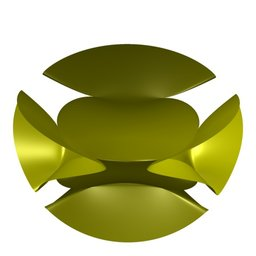
\includegraphics[height=1.2cm]{./../../common/images/barthquintic_green}
        &
        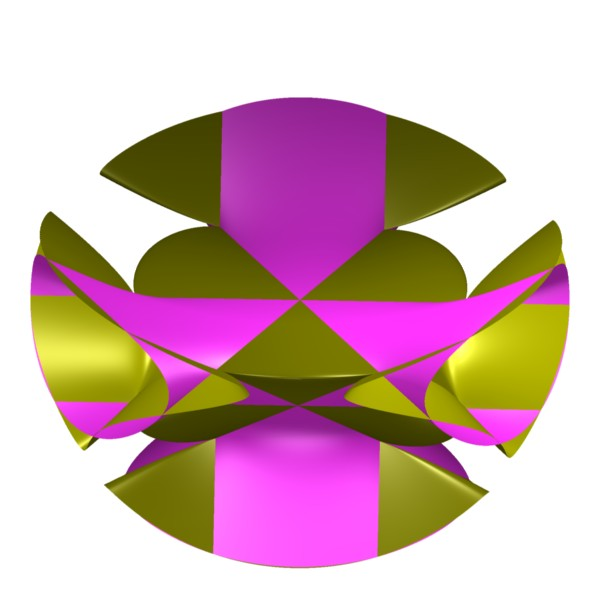
\includegraphics[height=1.2cm]{./../../common/images/barthquintic_clebschcubic}
        &
        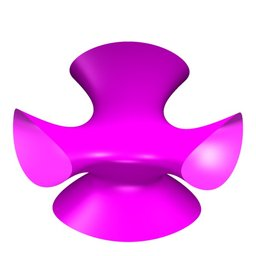
\includegraphics[height=1.2cm]{./../../common/images/clebschcubic_pink}
      \end{tabular}
    \end{center}
    \vspace*{-0.3em}
\end{surferPage}
